\title{Open Sound Control}
\author{
        Michael Lazarski \\
                Studiengang Media Systems\\
}
\date{\today}
\documentclass[a4paper, 12pt]{article}
\usepackage[ngerman]{babel}
\usepackage[utf8]{inputenc}
\usepackage{graphicx}
\usepackage{float}
\usepackage{url}
\usepackage{hyperref}
\usepackage{textcomp}
\usepackage{listings}

\pagestyle{headings}
\setcounter{secnumdepth}{5}
\begin{document}
\maketitle

\newpage
\tableofcontents
\newpage


\section{Geschichte}
\subsection{Musical Instrument Digital Interface}
Die Geschichte von Open Sound Control beginnt mit MIDI (Musical Instrument digital Interface).
Also am Anfang der 1980er große Synthesizer Manufakturen beginnen MIDI als Standard-Protokoll in ihre Hardware zu Implementieren wurde dies damals als eine Revolution in der Musikindustrie angesehen. Nur mit einem Computer, einem MIDI-Controller und der dazugehörigen Software konnte ein Musiker aufnehmen, komponieren und mischen ohne zusätzliches Werkezug. MIDI wird bis heute noch in der Musikindustrie benutzt.
\paragraph{Wie MIDI Funktioniert}

MIDI ist eine unidirektionale Schnittstelle zur seriellen Datenübertragung. MIDI hat keine Datenflusskontrolle. Die Übertragungsgeschwindigkeit beträgt 31250 Bit/s. \cite{MIDI} \\
\\
Es gibt 3 verschiedene MIDI-Anschlüsse \begin{itemize}
  \item MIDI-IN: Hiermit empfängt der MIDI-Controller Signale.
  \item MIDI-OUT: Hiermit sendet der MIDI-Controller Signale.
  \item MIDI-THRU: Sendet die ankommenden Signale vom MIDI-IN Port einfach weiter ohne sie weiter zu verarbeiten.
\end{itemize}
 \begin{figure}[htbp]
  \centering
  \fbox{
    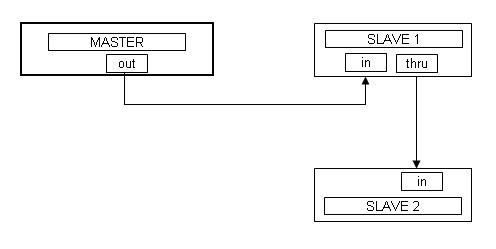
\includegraphics{mms.jpg}
  }
  \caption[MIDI Master Slave \cite{MMS}]{MIDI Master Slave}
  \label{fig:mms}
\end{figure}
MIDI funktioniert nach einem Master-Slave-Prinzip ~\ref{fig:mms}.
Will man mit einem MIDI-Keyboard (Master) einen Synthesizer (Slave) steuern, so verbindet man die MIDI-OUT Buchse des Masters mit der MIDI-IN Buchse des Slaves. Möchte man nun noch einen zweiten Slave hinzufügen, so schließt man ein Kabel zwischen dem MIDI-THRU des ersten Slaves mit der MIDI-IN Buchse des zweiten Slaves.

\subsubsection{Nachteile von MIDI}
Die Nachteile von MIDI sind:
\begin{itemize}
\item Serieller Transport der Daten. Die Daten müssen erst sequenziell geordnet werden.
  \item Langsame Übertragungsraten. Sehr problematisch bei großen Datenmengen.
  \item Pitch wird in Integern dargestellt.
  \item Tendiert zu Keyboard-Controllern da Wind, Gittern und andere Instrumente schwer zu Implementieren sind.
  \item Integer-Repräsentation von Controllerwerten. Dies kann zu Ungenauigkeit führen beim Einstellen von feinen Parametern.
  \item Ungenau Zeitauflösung, da diese in Integern angegeben wird.
  \item MIDI benötig spezielle Hardware.
\end{itemize}
\subsection {Zeta Instrument Processor Interface}
1994 wurde von der Firma Zeta Instruments und einer Forschungsgruppe der University of California das Zeta Instrument Processor Interface (kurz ZIPI) vorgestellt. Es sollte MIDI ablösen und war auf dem OSI-Model aufgebaut. ZIPI konnte sich nie wirklich durchsetzen. MIDI hat eine Peer-to-Peer-Architektur während ZIPI auf einer Stern Architektur mit einem HUB in der Mitte als zentrale Anlaufsstelle aufbaute. Das hatte den Vorteil, dass man einfach Geräte aus dem HUB entfernen konnte. Außerdem ist ZIPI auch unabhängig von einer physikalischen Implementierung. Das alles hat aber nicht geholfen, da das Adressierungsschema zu komplex war. Es mussten 1016127 Synth-Zustände geregelt werden im ZIPI Controller. Zum Vergleich hatte MIDI nur 16 Kanäle, die zwischen 12 und 128 zuständen hatten.
Es gibt bis heute keine kommerziell vertriebenen Geräte die ZIPI unterstützen.
\newpage
\section{Open Sound Control}
1997 kündigten die ZIPI Entwickler Matt Wright und Adrian Freed das Open Sound Protokoll an, auch bekannt unter dem Namen Open Sound Control. Es ist ein gutes Beispiel von modernen Netzwerk-Datenübertragungs-Kontrollsystemen. Wie andere Transportprotokolle erlaubt Open Sound Control es, dass die Kommunikation zwischen einem Computer und anderen Mediengeräten stattfinden kann, darüber hinaus ermöglicht Open Sound Control auch die Möglichkeit das Programme, die auf einem Gerät laufen, Daten miteinander austauschen können. Open Sound Control wurde speziell für Musiker entwickelt es kann aber auch gut in anderen Gebieten der netzwerkbasierten Kontrolle von System angewendet werden.

\subsection{Technik}
Einer der Vorteile von Open Sound Control ist, dass man dafür keine spezielle Hardware braucht, wie es z.B. bei MIDI der Fall ist. Open Sound Control unterstützt das Transmission Control Protocol TCP und das User Datagram Protocol UDP, die allgemein bekannt sind und z.B. im Internet oder im Heimnetzwerk schon verwendet werden. Dadurch hat Open Sound Control keine Geschwindigkeitsgrenze. Wir das Netzwerks schneller in dem Open Sound Control eingesetzt, so wird auch das Protokoll schneller verarbeitet. Durch diese Architektur könnte man Open Sound Control auch Open Stuff Control nennen, da theoretisch damit alles gesteuert werden kann, was eine Netzwerkschnittstelle hat.
\subsubsection{OSC Packets}
Die Nachrichten werden in sogenannten OSC Packets verschickt. Eine Applikation die OSC Pakete verschickt nennt man OSC-Client. Jede Applikation die OSC Packete empfängt nennt man OSC Server.
\\
Ein OSC Packet
\subsubsection{Transmission Control Protocol}
TCP ist ein verbindungsorientiertes Protokoll. Das heißt jeder Teilnehmer eines Netzwerkes kann exakt zurück verfolgt werden. Der direkte Austausch zweier Stellen ist gewährleistet und Datenverluste können behoben werden, da Daten neu angefordert werden können.

\subsubsection{User Datagram Protocol}
UDP ist ein verbindungsloses Protokoll. Heißt, Daten werden als “Stream” übertragen. Das heißt ein Sender beginnt “auf Glück” mit dem senden von Daten. Der Empfänger hat jedoch keine Möglichkeit eine Korrektur anzufordern. Der Vorteil von UDP: Es wird an alle Teilnehmer eines Netzwerkes gleichzeitig gesendet.
\subsection{Syntax}
\subsubsection{OSC-Message}
EditierenEine sogenannte OSC Message ist aufgeteilt in:
\begin{itemize}
  \item Address Pattern
  \item Type Tag String
  \item Arguments
\end{itemize}
\subsubsection{Adress Pattern}
Ein Open Sound Control Adress Pattern beginnt immer mit einem "/" (Forward Slash) gefolgt von einem String. Möchte man nun also einen Cutoff-Filter auf einem Synthesizer ändern, so kann man diesen mit:\\
\\
{\bf /synthesizer/filter/cutoff } \\
\\
ansprechen.
\subsubsection{Type Tag String}
Es gibt fünf "Atomic Data Types"\cite{OSCspec}. Diese sollten in jeder Open Sound Control Implementierung vorhanden sein.
\begin{itemize}
	\item int32 - 32-bit big-endian two's complement integer
	\item OSC-timetag - 64-bit big-endian fixed-point time tag, semantics defined below
	\item float32 - 32-bit big-endian IEEE 754 floating point number
	\item OSC-String - A sequence of non-null ASCII characters followed by a null, followed by 0-3 additional null characters to make the total number of bits a multiple of 32.
	\item OSC-blob - An int32 size count, followed by that many 8-bit bytes of arbitrary binary data, followed by 0-3 additional zero bytes to make the total number of bits a multiple of 32.
\end{itemize}
Es gibt auch Type-Tags die in vielen Implementierungen vorhanden sind aber nicht vom Standard gefordert werden. Hier eine kleine Auswahl\cite{OSCspec}:
\begin{itemize}
\item c - n ascii character, sent as 32 bits
\item r - 32 bit RGBA color
\item m - 4 byte MIDI message. Bytes from MSB to LSB are: port id, status byte, data1, data2
\item T - True. No bytes are allocated in the argument data.
\item F - False. No bytes are allocated in the argument data.
\item N - Nil. No bytes are allocated in the argument data.
\item I - Infinitum. No bytes are allocated in the argument data.
\item $ [ $  -Indicates the beginning of an array. The tags following are for data in the Array until a close brace tag is reached.
\item $ ] $ - Indicates the end of an array.
\end{itemize}

Somit ist jeder Typ ein vielfaches von 32 bit. Ein paar beispiel:\\
\\
{\bf /foo,f 440}\\
{\bf /foo,iisff 1000 -1 "hello" 1.23 4.56}\\

Wie man an den Beispielen sehen kann, kann man auch mehrere Argumente in einer Nachricht übergeben. Im zweiten Beispiel sind die Argumente 1000, -1, "hell" 1.23 4.56.
In einer Programmiersprache wie Java würde so eine Übergabe aussehen: \\
\\
{\bf foo(new Integer(1000), new Integer(-1),new String("hello"), new Float(1.23), new Float(4.56)}\\
\\
Die Nachricht in Byte Darstellung:
\begin{table}[ht]
\centering
\begin{tabular}{|p{0.5cm}|p{1.5cm}|p{0.5cm}|p{1.5cm}|p{0.5cm}|p{1.5cm}|p{0.5cm}|p{1.5cm}|}
\hline
 2f & (/) & 66 & (f) & 6f & (o) & 6f & (o)\\ \hline
 0 & () & 0 & () & 0 & () & 0 & ()\\ \hline
 2c & (,) & 69 & (i) & 69 & (i) & 73 & (s) \\ \hline
 66 & (f) & 66 & (f) & 0 & () & 0 & () \\ \hline
 0 & () & 0 & () & 3 & () & e8 & (è) \\ \hline
 ff & (ÿ) & ff & (ÿ) & ff & (ÿ) & ff & (ÿ) \\
 68 & (h) & 65 & (e) & 6c & (l) & 6c & (l) \\ \hline
 6f & (o) & 0 & () & 0 & () & 0 & () \\ \hline
 3f & (?) & 9d & () & f3 & (ó) & b6 & (¶) \\ \hline
 40 & (@) & b5 & (µ) & b2 & (”) & 2d & (-) \\ \hline
\end{tabular}
\end{table}
\newpage
An der Tabelle lässt sich gut die 32 Bit Aufteilung erkennen.

\section{Implementierungen}
\subsection{Hardware Implementierungen}
\subsubsection{The Missing Link OSC/MIDI Translator}

The Missing Link ist eine kleine unabhängige Box, die ihre eignes Wifi-Netzwerk aufbaut. So kann man mit mobilen Geräten auf die Box zugreifen. Sie übersetzt dann die speziellen OSC-Nachrichten in MIDI Nachrichten, mit der man z.B. Synthesizer kontrollieren kann. The Missing Link ist für schnelle Übertragungen, Flexibilität und Konfigurierbarkeit ausgelegt. Es braucht keinen Computer, der die Steuerung übernimmt. So kann OSC-fähige Wireless-Lan-Geräte direkt mit der Box kommunizieren. Es können sogar mehrere OSC Geräte auf die Box zugreifen.
\paragraph{Spezifikation}
\begin{itemize}
  \item 802.11b WiFi: adhoc oder infrastructure Modus und open, WEP, WPA oder WPA2 Sicherheit
  \item OSC über wireless UDP: OSC zu MIDI, MIDI zu OSC, Multiple gleichzeitige Verbindungen
  \item MIDI: MIDI IN/OUT (Standard 5 Pin). Konfigurierbares internes Routing mit soft MERGE/THRU. Alle MIDI befehle sind Implementiert.
  \item Strom: 9V-12V DC, tip +/-, >=250mA oder über USB
  \item Abmessungen: 3.3" x 2.2" x 1.6"
\begin{figure}[!htb]
  \centering
  \fbox{
    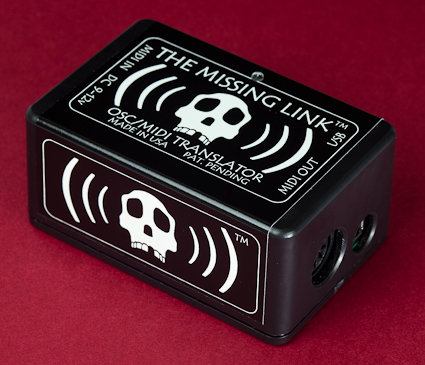
\includegraphics{themissinglink.jpg}
  }
  \caption[The Missing link \cite{TMLI}]{The Missing Link}
  \label{fig:TMLI}
\end{figure}
\end{itemize}
\subsection{Software Implementierungen}
\subsubsection{osc-ruby}
osc-ruby ist eine simple OSC 1.1 Implementierung für Ruby 1.9/2.0 und für JRuby.
Sie kann sowohl auf dem Client als auch auf dem Server eingesetzt werden.
Schauen wir uns eine simple Implementierung an, bei der ein Server und ein Client auf dem gleichen Host laufen.\cite{oscruby}
\newpage
\begin{lstlisting}[language=ruby]
# einbinden der Libary
require 'rubygems'
require 'osc-ruby'
require 'osc-ruby/em_server'
# Erstellen eines Serverobjektes
@server = OSC::EMServer.new( 3333 )
# Erstellen eines Client-Objektes der sich mit dem Server verbindet
@client = OSC::Client.new( 'localhost', 3333 )
# Implementierung einer einfachen Willkommensnachricht
@server.add_method '/greeting' do | message |
  puts "#{message.ip_address}:#{message.ip_port} -- #{message.address} -- #{message.to_a}"
end

# Starten des Server Loops
Thread.new do
  @server.run
end
# Ein "Willkommen!" an alle schicken
@client.send( OSC::Message.new( "/greeting" , "Willkommen!" ))
# nach 3 millisekunden das Program beenden
sleep( 3 )
\end{lstlisting}

\subsubsection{oscmex}
Mit oscmex gibt es eine Bibliothek die Funktionen für Matlab bereitstellt.
So können mit oscmex Nachrichten empfangen und gesendet werden zwischen OSC Endpunkten.
Die Libary ist dafür gedacht Musik zu analysieren. oscmex ist in C geschrieben.
Eine möglicher Einsatz wäre streng mathematische und genaue Gestensteuerung oder die genaue Berechnung von Timings für Präsentationen. Auf ein Beispiel wird verzichtet.\cite{oscmex}
\subsubsection{TouchOSC}
\begin{figure}[!htb]
  \centering
  \fbox{
    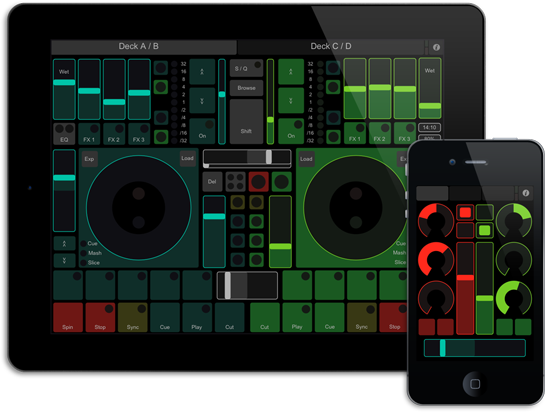
\includegraphics[width=13.5cm]{tochosc.png}
  }
  \caption[TouchOSC \cite{touchosc}]{TouchOSC}
  \label{fig:touchosc}
\end{figure}
TouchOSC ist eine Applikation für Apples iOS und Googles Android. Für beide Systeme kostet sie 4,99\$. Das Besondere an TouchOSC ist das es Nachrichten über Wireless LAN verschicken und empfangen kann. Dadurch eignet sich TouchOSC besonders für Live-Auftritte oder Live-Shows. Ein voller MIDI und Apples Logic Pro Support ist implementiert. TouchOSC ist komplett modular so kann es z.B. als DJ pult oder als Effektgeräte oder als Drum-Synthesizer genutzt werden. Frei erhältlich ist ein Interface-Editor so kann man am Computer sein Interface erstellen und abspeichern, damit es zu einem späteren Zeitpunkt wiederbenutzt werden kann.
\newpage
\renewcommand{\refname}{REFERENCES}
\bibliographystyle{plainnat}
\bibliography{evt}

\listoffigures
\end{document}

